%!Mode:: "TeX:UTF-8"
\documentclass[a4paper,11pt,UTF8]{ctexart}

\usepackage{indentfirst} %缩进
\usepackage{xeCJK}    %使用系统字体
\usepackage{fancyhdr} %自定义页眉页脚
\pagestyle{empty}                   %不设置页眉页脚
\usepackage{amsmath, amsthm, amssymb, amsfonts} %数学公式
\usepackage[a4paper,left=3cm,right=3cm,top=3cm,bottom=3cm]{geometry}
%\usepackage[tmargin=1in,bmargin=1in,lmargin=1.25in,rmargin=1.25in]{geometry}.
\usepackage{booktabs} %插入表格
\usepackage[section]{placeins} %避免浮动
\usepackage{listings} %插入代码
\usepackage{ctex}     %中文宏包
\usepackage[svgnames, table]{xcolor} %彩色表格
\usepackage{algorithm}          %伪代码
\usepackage{algorithmicx}
\usepackage{algpseudocode}
\usepackage{algorithm,algpseudocode,float}
\usepackage{lipsum}
\usepackage{enumitem}           %调整列举环境
\usepackage{url}
\usepackage{float}
\usepackage{upgreek}
\usepackage{fontspec,xunicode}
\defaultfontfeatures{Mapping=tex-text} %如果没有它,会有一些 tex 特殊字符无法正常使用,比如连字符。

\usepackage{graphicx}
\graphicspath{{imgs/}}

%%%%%%%%%%%%%%%%%%%%%%%%%%%%%%%%%%%%%%%%%%%%%%%%%%%%%%%%%%%%%%%%
% 缩进及行间距
%%%%%%%%%%%%%%%%%%%%%%%%%%%%%%%%%%%%%%%%%%%%%%%%%%%%%%%%%%%%%%%%
\setlength{\parindent}{22pt} %重新定义缩进长度
\setlength{\baselineskip}{20pt}  %定义行间距
%\renewcommand{\baselinestretch}{1.1} %定义行间距

%%%%%%%%%%%%%%%%%%%%%%%%%%%%%%%%%%%%%%%%%%%%%%%%%%%%%%%%%%%%%%%%
% 列表设置
%%%%%%%%%%%%%%%%%%%%%%%%%%%%%%%%%%%%%%%%%%%%%%%%%%%%%%%%%%%%%%%%
\setenumerate{fullwidth,itemindent=\parindent,listparindent=\parindent,itemsep=0ex,partopsep=0pt,parsep=0ex}
\setenumerate[2]{label=\alph*),leftmargin=1.5em}  %二级item设置
\setitemize{itemindent=38pt,leftmargin=0pt,itemsep=-0.4ex,listparindent=26pt,partopsep=0pt,parsep=0.5ex,topsep=-0.25ex}
\setdescription{itemindent=38pt,leftmargin=0pt,itemsep=-0.4ex,listparindent=26pt,partopsep=0pt,parsep=0.5ex,topsep=-0.25ex}

%%%%%%%%%%%%%%%%%%%%%%%%%%%%%%%%%%%%%%%%%%%%%%%%%%%%%%%%%%%%%%%%
% 图的标题行间距设置
%%%%%%%%%%%%%%%%%%%%%%%%%%%%%%%%%%%%%%%%%%%%%%%%%%%%%%%%%%%%%%%%
\newcommand{\bottomcaption}{%
\setlength{\abovecaptionskip}{6pt}%
\setlength{\belowcaptionskip}{6pt}%
\caption}


%%%%%%%%%%%%%%%%%%%%%%%%%%%%%%%%%%%%%%%%%%%%%%%%%%%%%%%%%%%%%%%%
% 字体定义
%%%%%%%%%%%%%%%%%%%%%%%%%%%%%%%%%%%%%%%%%%%%%%%%%%%%%%%%%%%%%%%%
\setmainfont{Times New Roman}  %默认英文字体.serif是有衬线字体sans serif无衬线字体
\setmonofont{Consolas}
\setCJKmainfont[ItalicFont={楷体}, BoldFont={黑体}]{宋体}%衬线字体 缺省中文字体为
\setCJKsansfont{黑体}
\punctstyle{hangmobanjiao}
%-----------------------xeCJK下设置中文字体------------------------------%
\setCJKfamilyfont{song}{SimSun}                             %宋体 song
\newcommand{\song}{\CJKfamily{song}}
\setCJKfamilyfont{fs}{FangSong}                      %仿宋  fs
\newcommand{\fs}{\CJKfamily{fs}}
\setCJKfamilyfont{ktgb}{KaiTi}                      %楷体2312 ktgb
\newcommand{\ktgb}{\CJKfamily{ktgb}}
\setCJKfamilyfont{yh}{Microsoft YaHei}                    %微软雅黑 yh
\newcommand{\yh}{\CJKfamily{yh}}
\setCJKfamilyfont{hei}{SimHei}                              %黑体  hei
\newcommand{\hei}{\CJKfamily{hei}}
\setCJKfamilyfont{hwxk}{STXingkai}                                %华文行楷  hwxk
\newcommand{\hwxk}{\CJKfamily{hwxk}}
%------------------------------设置字体大小------------------------%
\newcommand{\shiyanbaogao}{\fontsize{36pt}{\baselineskip}\selectfont}
\newcommand{\chuhao}{\fontsize{42pt}{\baselineskip}\selectfont}     %初号
\newcommand{\xiaochuhao}{\fontsize{36pt}{\baselineskip}\selectfont} %小初号
\newcommand{\yihao}{\fontsize{28pt}{\baselineskip}\selectfont}      %一号
\newcommand{\erhao}{\fontsize{21pt}{\baselineskip}\selectfont}      %二号
\newcommand{\xiaoerhao}{\fontsize{18pt}{\baselineskip}\selectfont}  %小二号
\newcommand{\sanhao}{\fontsize{15.75pt}{\baselineskip}\selectfont}  %三号
\newcommand{\sihao}{\fontsize{14pt}{\baselineskip}\selectfont}       %四号
\newcommand{\xiaosihao}{\fontsize{12pt}{\baselineskip}\selectfont}  %小四号
\newcommand{\wuhao}{\fontsize{10.5pt}{\baselineskip}\selectfont}    %五号
\newcommand{\xiaowuhao}{\fontsize{9pt}{\baselineskip}\selectfont}   %小五号
\newcommand{\liuhao}{\fontsize{7.875pt}{\baselineskip}\selectfont}  %六号
\newcommand{\qihao}{\fontsize{5.25pt}{\baselineskip}\selectfont}    %七号

%%%%%%%%%%%%%%%%%%%%%%%%%%%%%%%%%%%%%%%%%%%%%%%%%%%%%%%%%%%%%%%%
% 图题字体大小相同
%%%%%%%%%%%%%%%%%%%%%%%%%%%%%%%%%%%%%%%%%%%%%%%%%%%%%%%%%%%%%%%%
\usepackage{caption}
\captionsetup{font={footnotesize}}   % footnotesize = 9pt
\captionsetup[lstlisting]{font={footnotesize}}

%%%%%%%%%%%%%%%%%%%%%%%%%%%%%%%%%%%%%%%%%%%%%%%%%%%%%%%%%%%%%%%%
% 重定义枚举编号为 1),2)...
%%%%%%%%%%%%%%%%%%%%%%%%%%%%%%%%%%%%%%%%%%%%%%%%%%%%%%%%%%%%%%%%
\renewcommand{\labelenumi}{\theenumi)}

%%%%%%%%%%%%%%%%%%%%%%%%%%%%%%%%%%%%%%%%%%%%%%%%%%%%%%%%%%%%%%%%
% 标题名称中文化
%%%%%%%%%%%%%%%%%%%%%%%%%%%%%%%%%%%%%%%%%%%%%%%%%%%%%%%%%%%%%%%%
\renewcommand\figurename{\hei 图}
\renewcommand\tablename{\hei 表}
\renewcommand\lstlistingname{\hei 代码}
\renewcommand{\algorithmicrequire}{\textbf{输入:}}
\renewcommand{\algorithmicensure}{\textbf{输出:}}
\newtheorem{define}{定义}

%%%%%%%%%%%%%%%%%%%%%%%%%%%%%%%%%%%%%%%%%%%%%%%%%%%%%%%%%%%%%%%%
% 代码设置
%%%%%%%%%%%%%%%%%%%%%%%%%%%%%%%%%%%%%%%%%%%%%%%%%%%%%%%%%%%%%%%%
\lstset{
 columns=fixed,
 numbers=left,                                        % 在左侧显示行号
 numberstyle=\tiny\color{gray},                       % 设定行号格式
 frame=single,                                        % 单线背景边框
 breaklines=true,                                     % 设定LaTeX对过长的代码行进行自动换行
 keywordstyle=\color[RGB]{40,40,255},                 % 设定关键字颜色
 numberstyle=\footnotesize\color{darkgray},
 commentstyle=\it\color[RGB]{0,96,96},                % 设置代码注释的格式
 stringstyle=\rmfamily\slshape\color[RGB]{128,0,0},   % 设置字符串格式
 showstringspaces=false,                              % 不显示字符串中的空格
 language=java,                                        % 设置语言
 basicstyle=\linespread{1.0}\xiaowuhao\ttfamily,                      % 字体字号
 %lineskip=10pt,
 %baselinestretch=1,
}
%%%%
\newcommand\mr[1]{\mathrm{#1}}
\newcommand\dd{\mathrm{d}}
%%%%
%%%%%%%%%%%%%%%%%%%%%%%%%%%%%%%%%%%%%%%%%%%%%%%%%%%%%%%%%%%%%%%%
% 伪代码分页
%%%%%%%%%%%%%%%%%%%%%%%%%%%%%%%%%%%%%%%%%%%%%%%%%%%%%%%%%%%%%%%%
\makeatletter
\renewcommand{\ALG@name}{算法}
\newenvironment{breakablealgorithm}
  {% \begin{breakablealgorithm}
   \begin{center}
     \refstepcounter{algorithm}% New algorithm
     \hrule height.8pt depth0pt \kern2pt% \@fs@pre for \@fs@ruled
     \renewcommand{\caption}[2][\relax]{% Make a new \caption
       {\raggedright\textbf{\ALG@name~\thealgorithm} ##2\par}%
       \ifx\relax##1\relax % #1 is \relax
         \addcontentsline{loa}{algorithm}{\protect\numberline{\thealgorithm}##2}%
       \else % #1 is not \relax
         \addcontentsline{loa}{algorithm}{\protect\numberline{\thealgorithm}##1}%
       \fi
       \kern2pt\hrule\kern2pt
     }
  }{% \end{breakablealgorithm}
     \kern2pt\hrule\relax% \@fs@post for \@fs@ruled
   \end{center}
  }
\makeatother

% =============================================
% Part 1 Edit the info
% =============================================

\newcommand{\major}{物理学院}
\newcommand{\name}{黄阅迅,李秋阳}
\newcommand{\stuid}{PB18020631,PB18020567}
\newcommand{\group}{20}
\newcommand{\newdate}{\today}


\newcommand{\course}{电子线路实验(1)}
\newcommand{\newtitle}{集成运放应用——模拟运算电路}

% =============================================
% Part 1 Main document
% =============================================
\begin{document}
\thispagestyle{empty}
\begin{figure}[h]
  \begin{minipage}{0.6\linewidth}
    \centerline{
\includegraphics[width=\linewidth]{logo.png}}
  \end{minipage}
  \hfill
  \begin{minipage}{.4\linewidth}
    \raggedleft
    \begin{tabular*}{.8\linewidth}{ll}
      学院: & \underline\major   \\
      姓名: & \underline\name    \\
      学号: & \underline\stuid   \\
      组号:  & \underline\group   \\
      日期: & \underline\newdate \\
    \end{tabular*}
  \end{minipage}
\end{figure}

\begin{table}[!htbp]
  \centering
  \begin{tabular*}{\linewidth}{llllll}
    课程名称:  \underline\course   \qquad\qquad 实验题目:  \underline\newtitle  
  \end{tabular*}
\end{table}

% =============================================
% Part 2 Main document
% =============================================

\section{实验目的}

请参见预习报告。

\section{实验原理}

请参见预习报告。

\section{实验内容与步骤}
\subsection{实验一:反向比例运算电路}
 实验电路如图\ref{fig:Exp01}所示:
 \begin{figure}[H]
  \centering
  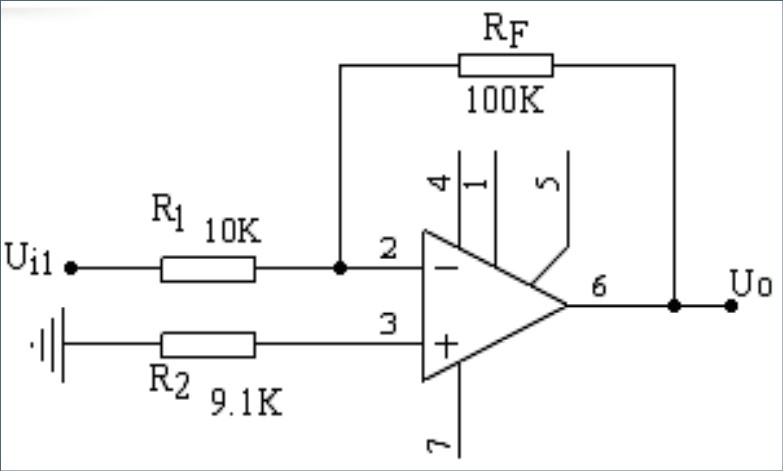
\includegraphics[width=6cm]{Exp01Circ}
  \caption{实验一电路图}
  \label{fig:Exp01}
 \end{figure}
 输入 $f=500\mr{Hz},~V_i=0.5\mr{V_{rms}}$ 的正弦交流信号,
用示波器测量 $V_i$、 $V_o$ 有效值,并观察 $V_o$ 和 $V_i$ 的相位关系,画出大概的输入输出波形来表征相位。
\subsection{实验二:反向加法运算电路}
 实验电路图如图\ref{fig:Exp02}所示:
 \begin{figure}[H]
  \centering
  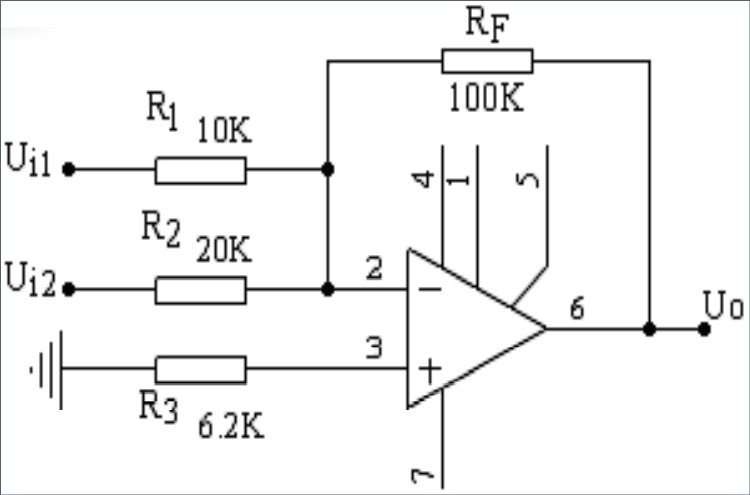
\includegraphics[width=6cm]{Exp02Circ}
  \caption{实验二电路图}
  \label{fig:Exp02}
 \end{figure}
 $V_{i1}$ 和 $V_{i1}$ 是直流稳压电源,用万用表DCV档测量 $V_{i1},~V_{i2}$ 和 $V_o$ 。
 \subsection{实验三:同相比例运算电路}
 实验电路图如图\ref{fig:Exp03}所示:
 \begin{figure}[H]
  \centering
  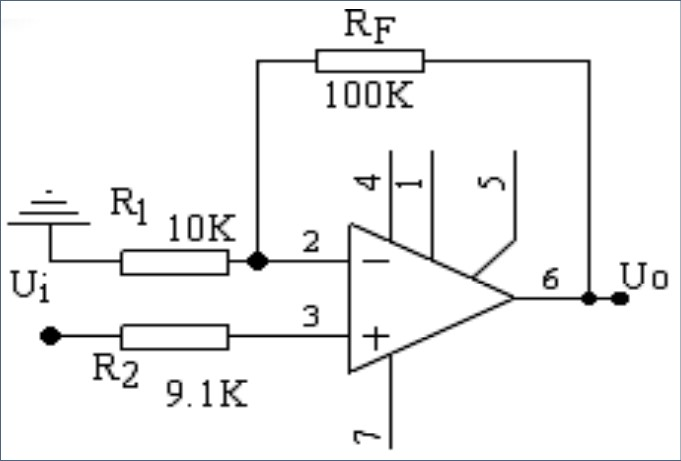
\includegraphics[width=6cm]{Exp03Circ}
  \caption{实验三电路图}
  \label{fig:Exp03}
 \end{figure}
 输入 $f=500\mr{Hz},~V_i=0.5\mr{V_{rms}}$ 的正弦交流信号,
用示波器测量 $V_i$、 $V_o$ 有效值,并观察 $V_o$ 和 $V_i$ 的相位关系,画出大概的输入输出波形来表征相位。
 \subsection{实验四:差动放大电路(减法器)}
 实验电路图如图\ref{fig:Exp04}所示:
 \begin{figure}[H]
  \centering
  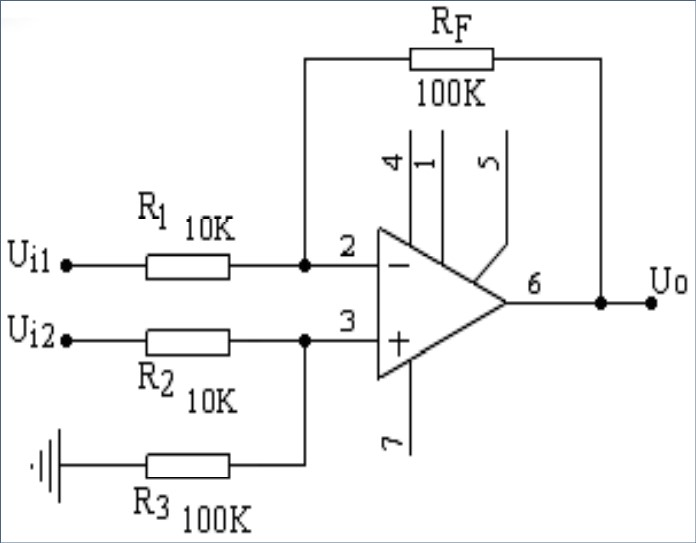
\includegraphics[width=6cm]{Exp04Circ}
  \caption{实验四电路图}
  \label{fig:Exp04}
 \end{figure}
 $V_{i1}$ 和 $V_{i1}$ 是直流稳压电源,用万用表DCV档测量 $V_{i1},~V_{i2}$ 和 $V_o$ 。注意输入电压不能太大,防止 $V_o$ 进入饱和区。
 \subsection{实验五:积分运算电路}
 实验电路图如图\ref{fig:Exp05}所示:
 \begin{figure}[H]
  \centering
  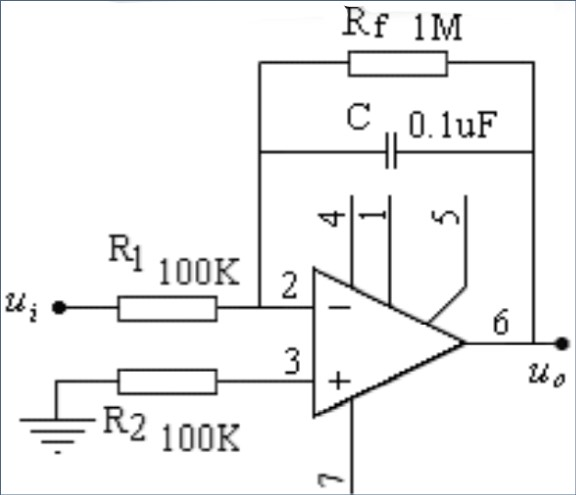
\includegraphics[width=6cm]{Exp05Circ}
  \caption{实验五电路图}
  \label{fig:Exp05}
 \end{figure}
 输入信号为 $f=100\mr{Hz}$ ,峰峰值为 $2\mr{V}$ 的方波信号,画出 $V_i,~V_o$ 波形,计算 $V_{opp}$ 的实际值与理论值。
 \subsection{实验六:微分运算电路}
 实验电路图如图\ref{fig:Exp06}所示:
 \begin{figure}[H]
  \centering
  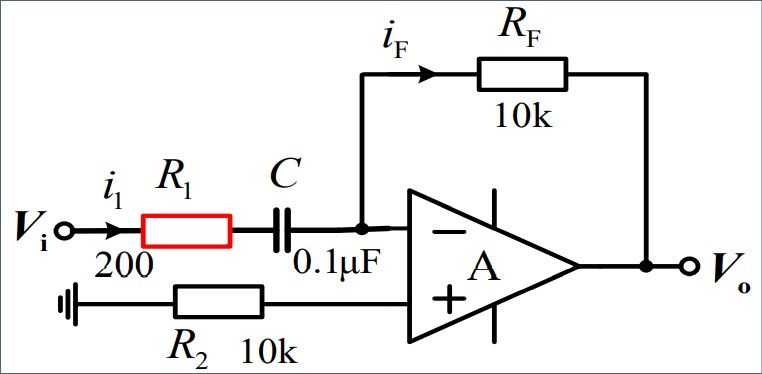
\includegraphics[width=6cm]{Exp06Circ}
  \caption{实验六电路图}
  \label{fig:Exp06}
 \end{figure}
 输入信号为 $f=100\mr{Hz}$ ,峰峰值为 $2\mr{V}$ 的方波信号,画出 $V_i,~V_o$ 波形。
 
\section{实验数据处理与分析}
\subsection{实验一:反向比例运算电路}
\subsubsection{实验数据}
电路元件参数:
\[ R_1=9.769\mr{k}\Omega,~R_2=8.969\mr{k}\Omega,~R_F=102.2\mr{k}\Omega. \]
\par 输入输出电压以及放大系数:
\[ \mr{Theo}\,A_v=-\frac{R_F}{R_1}=-10.46 \]
\begin{table}[H]
 \centering
 \begin{tabular}{|r|r|r|r|}
 \hline
  $V_i(\mr{V_{rms}})$ &$V_o(\mr{V_{rms}})$ &$\mr{Exp}\,A_v$ 
  &$\mr{Theo}\,A_v$
  \\\hline
  0.5007 &5.212 &-10.41 &-10.46
  \\\hline
 \end{tabular}
 \caption{实验一数据}
\end{table}
\par 大致的输入输出波形:
\begin{figure}[H]
 \centering
 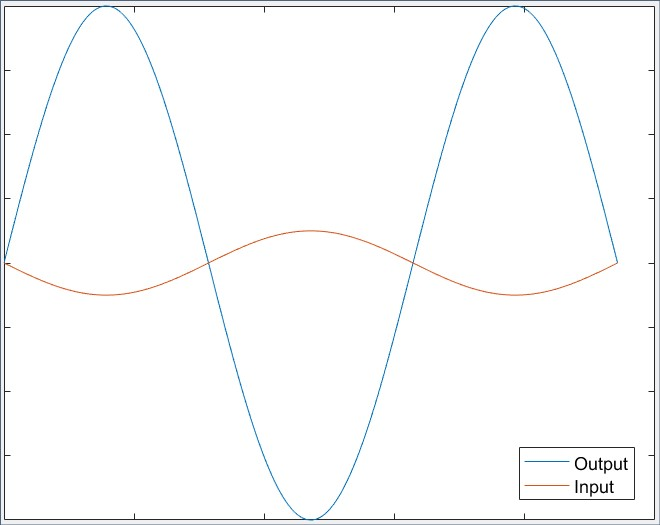
\includegraphics[width=8cm]{Exp01Wave}
 \caption{实验一的大致波形}
 \label{fig:Exp01Wave}
\end{figure}
\subsubsection{实验分析}
理论放大系数与实际放大系数很接近。从波形明显可以看出来,输出电压是被反相放大的,这与理论推导一致。

\subsection{实验二:反向加法运算电路}
电路元件参数:
\[ R_1=9.769\mr{k}\Omega,~R_2=20.14\mr{k}\Omega,~R_3=6.112\mr{k}\Omega,~R_F=102.2\mr{k}\Omega \]
输入输出电压以及放大系数:
\[ \mr{Theo}\,V_o=-\left( \frac{R_F}{R_1}V_{i1}+\frac{R_F}{R_2}V_{i2} \right)=-(10.462V_{i1}+5.074V_{i2}) \]
\begin{table}[H]
 \centering
 \begin{tabular}{|r|r|r|r|r|}
 \hline
  $V_{i1}(\mr{V})$ &0.1023 &0.3011 &-0.1016 &-0.3008
  \\\hline
  $V_{i2}(\mr{V})$ &0.2010 &0.6007 &-0.2012 &-0.6006
  \\\hline
  $\mr{Exp}\,V_o(\mr{V})$ &-2.137 &-6.244 &2.035 &6.145
  \\\hline
  $\mr{Theo}\,V_o(\mr{V})$ &-2.091 &-6.198 &2.084 &6.194
  \\\hline
  相对误差(\%) &2.200 &0.742 &2.351 &0.791
  \\\hline
 \end{tabular}
 \caption{实验二数据}
\end{table}
\subsubsection{实验分析}
该电路确实做到了反相加法。准确地说,是对两个输入电压进行反相线性组合。
\par 输出电压的相对误差不是很大,绝对误差都保持在0.05V左右,而且实际输出电压电位总是比理论输出电压低。
\par 考虑到输出电压的绝对误差接近一个定值,这个误差很有可能来源于运放正负端子之间的电压差。因为正负端子间并没有做到绝对的虚短,所以二者之间可能会有一个固定的电压差,从而导致实际输出电压总比理论值低一些。考虑到电路的特性,两个输入端的电流必定同向,那么这个电压偏移对输出电压的影响大致是一个常数。

\subsection{实验三:同相比例运算电路}
\subsubsection{实验数据}
电路元件参数:
\[ R_1=9.769\mr{k}\Omega,~R_2=8.969\mr{k}\Omega,~R_F=102.2\mr{k}\Omega. \]
\par 输入输出电压以及放大系数:
\[ \mr{Theo}\,A_v=1+\frac{R_F}{R_1}=11.46 \]
\begin{table}[H]
 \centering
 \begin{tabular}{|r|r|r|r|}
 \hline
  $V_i(\mr{V_{rms}})$ &$V_o(\mr{V_{rms}})$ &$\mr{Exp}\,A_v$ 
  &$\mr{Theo}\,A_v$
  \\\hline
  0.5010 &5.741 &11.46 &11.46
  \\\hline
 \end{tabular}
 \caption{实验三数据}
\end{table}
大致的输入输出波形:
\begin{figure}[H]
 \centering
 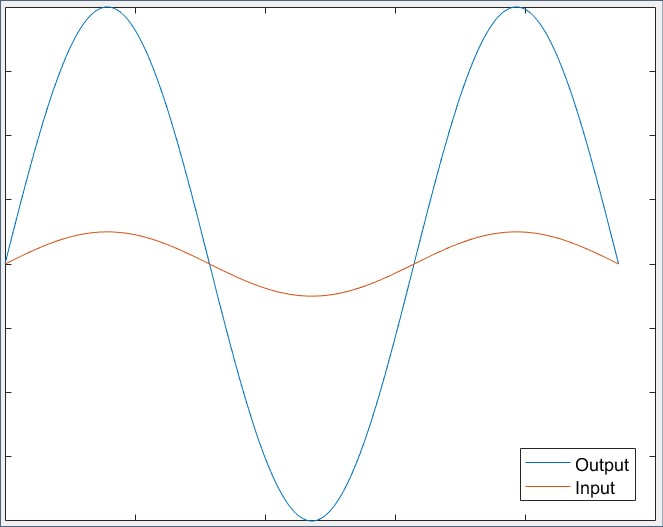
\includegraphics[width=8cm]{Exp03Wave}
 \caption{实验三的大致波形}
 \label{fig:Exp03Wave}
\end{figure}
\subsubsection{实验分析}
理论放大系数与实际放大系数很接近。从波形明显可以看出来,输出电压是被同相放大的,这与理论推导一致。

\subsection{实验四:差动放大电路(减法器)}
电路元件参数:
\[ R_1=9.769\mr{k}\Omega,~R_2=9.841\mr{k}\Omega,~R_3=101.0\mr{k}\Omega,~R_F=102.2\mr{k}\Omega \]
输入输出电压以及放大系数:
\[ \mr{Theo}\,V_o=\frac{R_F}{R_1}(V_{i2}-V_{i1})
=10.46(V_{i2}-V_{i1}) \]
\begin{table}[H]
 \centering
 \begin{tabular}{|r|r|r|r|r|}
 \hline
  $V_{i1}(\mr{V})$ &1.001 &2.001 &-1.001 &-2.001
  \\\hline
  $V_{i2}(\mr{V})$ &0.5007 &1.701 &-0.5007 &-1.701
  \\\hline
  $\mr{Exp}\,V_o(\mr{V})$ &-5.274 &-3.196 &5.205 &3.129
  \\\hline
  $\mr{Theo}\,V_o(\mr{V})$ &-5.233 &-3.138 &5.233 &3.138
  \\\hline
  相对误差(\%) &0.783 &1.848 &0.535 &0.287
  \\\hline
 \end{tabular}
 \caption{实验四数据}
\end{table}
\subsubsection{实验分析}
该电路是差动放大电路,输出电压值正比于两输入电压之差。
\par 可以看到,输出电压的相对误差很小。但是绝对误差有着和实验二不同的趋势:若输入电压中 $V_{i1}$ 较大,那么实验值低于理论值;若输入电压种 $V_{i2}$ 较大,那么实验值高于理论值。
\par 在实验二中已经给出了因运放不理想而导致的误差。此外我们发现,因为 $R_1=R_2,~R_3=R_F$ 不严格成立,所以理论计算式就需要作出修改。
\par 重新计算表达式为:
\[ V_o=\frac{R_3(R_F+R_1)}{R_1(R_2+R_3)}V_{i2}-\frac{R_F}{R_1}V_{i1}=10.44V_{i1}-10.46V_{i2} \]
\par 由此修正的结果为:
\begin{table}[H]
 \centering
 \begin{tabular}{|r|r|r|r|r|}
 \hline
  $V_{i1}(\mr{V})$ &1.001 &2.001 &-1.001 &-2.001
  \\\hline
  $V_{i2}(\mr{V})$ &0.5007 &1.701 &-0.5007 &-1.701
  \\\hline
  $\mr{Exp}\,V_o(\mr{V})$ &-5.243 &-3.172 &5.243 &3.172
  \\\hline
  $\mr{Theo}\,V_o(\mr{V})$ &-5.233 &-3.138 &5.233 &3.138
  \\\hline
  绝对误差($\mr{V}$) &-0.01 &-0.034 &0.01 &0.034
  \\\hline
 \end{tabular}
 \caption{实验四数据}
\end{table}
\par 虽然绝对误差未必被缩小了,但是现在,假如让 $V_{i1},~V_{i2}$ 同时反相,那么绝对误差的大小不变,仅符号变化。
\par 这看起来与实验二分析时给出的假设是矛盾的,我们给出一种可能的解释。运放肯定不是理想的,其正负端子间有电压差,端子间有小电流存在。如图\ref{fig:Exp04Ana},在实验二的情况下,$V_{i1},~V_{i2}$ 接在一个端子上,而且输入电压同符号,那么端子需要流入/流出更大的电流,因此正负端子间的压差比较大;而在实验四的情况下,$V_{i1},~V_{i2}$ 接在两个端子上,而且从电路看,输入电压端口的电流是同向的,也就是说,正负两个端子需要分别流入/流出差不多大的电流,因此正负端子间的压差会很小。
\begin{figure}[H]
 \centering
 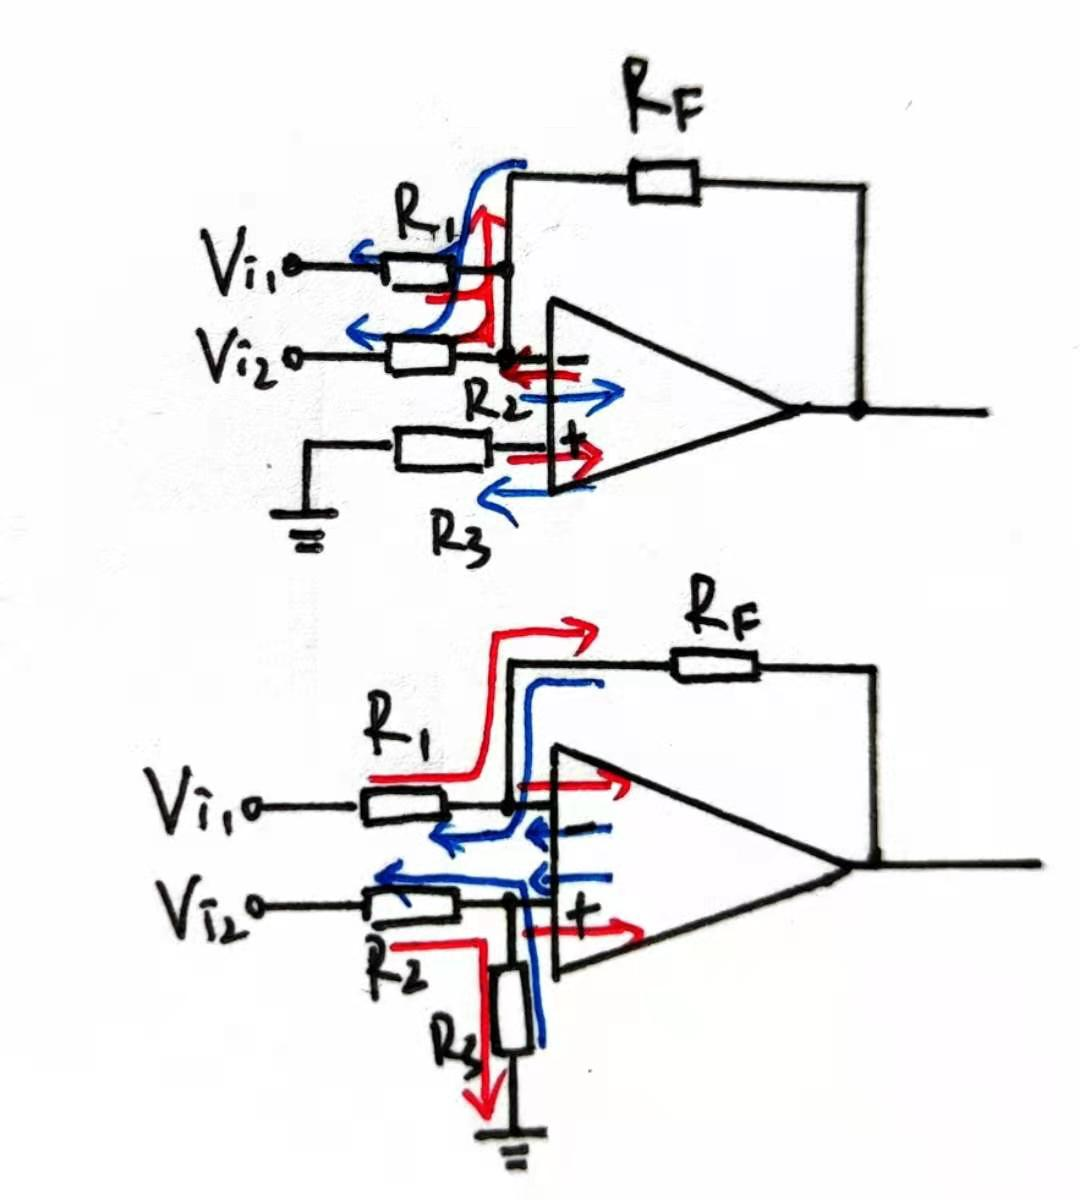
\includegraphics[width=4cm]{Exp04Ana}
 \caption{解释误差来源的示意图,红色蓝色分别为两端口电压同取正或负时的电流流向}
 \label{fig:Exp04Ana}
\end{figure}

\par 至于依然有 0.01-0.03V 的误差,是由于其他因素,诸如仪器因素、测量因素等等导致的,但是这和以上把正负电压都向大或向小改变的运放误差不是一种类型。
\par 上述分析也印证了差分式输入的一个优势:可以排除各种因素对信号的影响,因为如果两个输入信号被同向改变了同样的值,那么在差分输出段,这个误差会因减法消去。

\subsection{实验五:积分运算电路}
\subsubsection{实验数据}
电路元件参数:
\[ R_1=98.92\mr{k}\Omega,~R_2=101.0\mr{k}\Omega,~R_F=1.026\mr{M}\Omega,~C=0.095\mr{\upmu F} \]
\par 输入波形:
\begin{figure}[H]
 \centering
 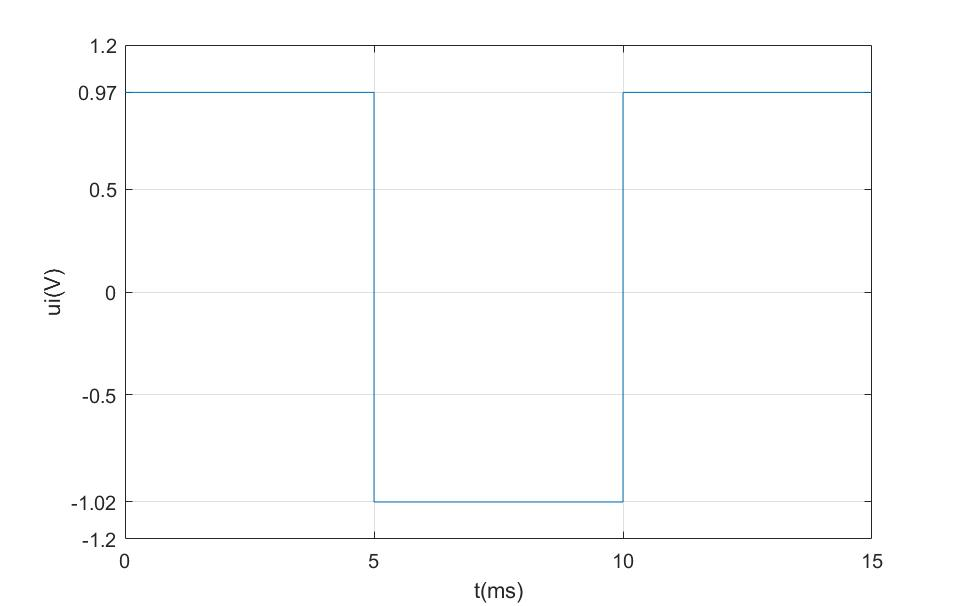
\includegraphics[width=10cm]{Exp05In}
 \caption{实验五输入波形}
 \label{fig:Exp05In}
\end{figure}
输出波形:
\begin{figure}[H]
 \centering
 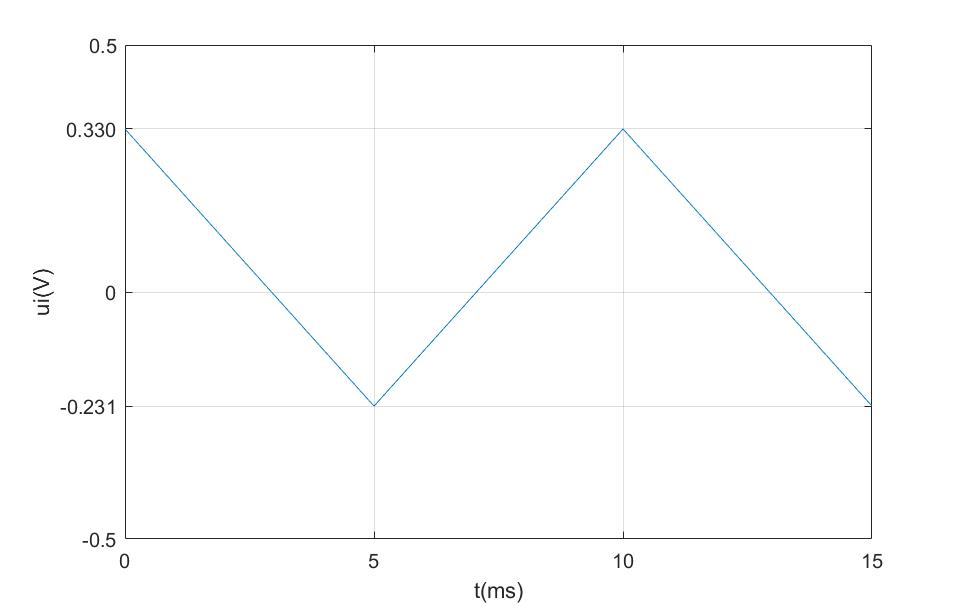
\includegraphics[width=10cm]{Exp05Out}
 \caption{实验五输出波形}
 \label{fig:Exp05Out}
\end{figure}
\subsubsection{实验分析}
理论下降沿峰峰值为:
\[ \tau=R_1C=98.92\mr{k}\Omega\times 0.095\mr{\upmu F}
 =9.3974\mr{ms} \]
\[ \Delta V_{pp}=-\frac{1}{R_1C}\int_0^tv_i(t)\dd{t}
 = -\frac{0.97\times 5}{9.3974}=-0.516\mr{V} \]
理论上升沿峰峰值为:
\[ \Delta V_{pp}=-\frac{1}{R_1C}\int_0^tv_i(t)\dd{t}
 = \frac{1.02\times 5}{9.3974}=0.543\mr{V} \]
\par 理论上讲,输出并非完美的三角波,每隔一个周期,峰值会往上加约 0.03V 。但是在示波器上本来只显示了二到三个周期,而且本身图线的线宽也不小,所以这种差别并不能用肉眼显著地看出来。
\par 实际上的峰峰值为:
\[ 0.330-(-0.231)=0.561\mr{V} \]
\par 这个值比理论的上升或下降沿值都大。误差为:
\[ \text{绝对误差:}|0.561-\frac{0.516+0.543}{2}|=0.0315\mr{V} \]
\[ \text{相对误差:}\frac{0.0315}{(0.516+0.543)/2}\times100\%  =5.95\% \]
\par 相对误差略大,但仍在可以接受的范围。
\par 而绝对误差在 0.03V 左右,这个误差并非很大。考虑到示波器在图线上手动定标带来的误差,以及图线的宽度,以及波形并非完美的三角波等等因素,这个绝对误差是可以接受的。

\subsection{实验六:微分运算电路}
\subsubsection{实验数据}
电路元件参数:
\[ R_1=163.2\Omega,~R_2=9.841\mr{k}\Omega,~R_F=9.722\mr{k}\Omega,~C=0.095\mr{\upmu F} \]
\par 输入波形:
\begin{figure}[H]
 \centering
 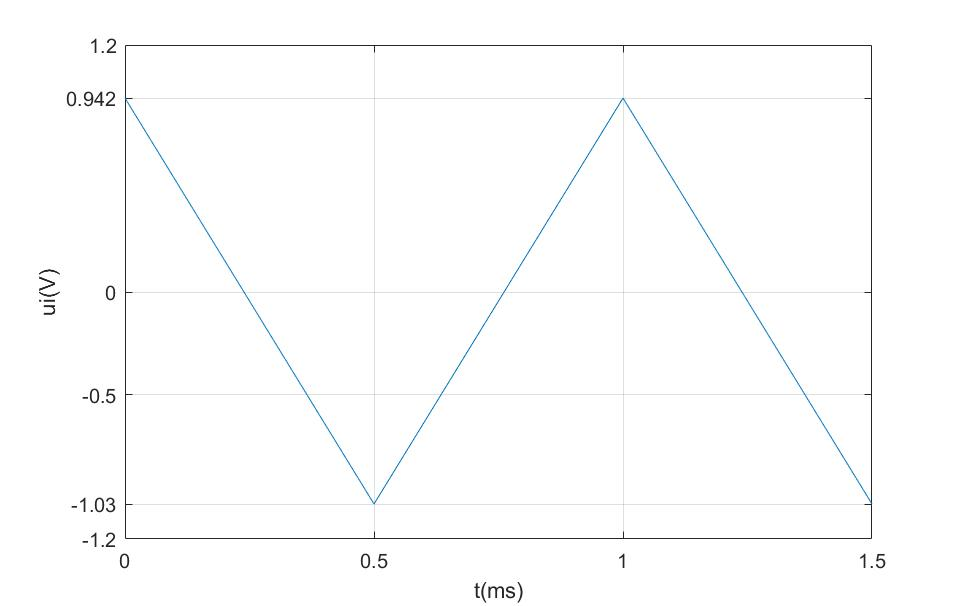
\includegraphics[width=10cm]{Exp06In}
 \caption{实验六输入波形}
 \label{fig:Exp06In}
\end{figure}
输出波形:
\begin{figure}[H]
 \centering
 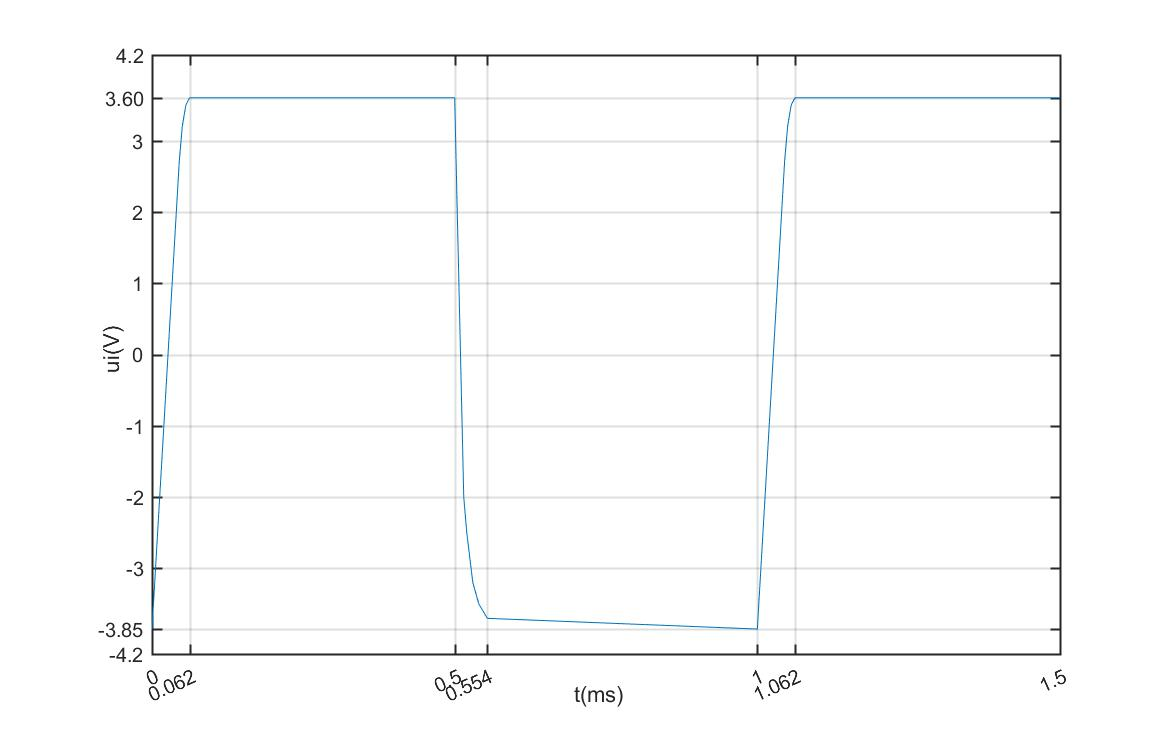
\includegraphics[width=10cm]{Exp06Out}
 \caption{实验六输出波形}
 \label{fig:Exp06Out}
\end{figure}
示波器波形的实际照片:
\begin{figure}[H]
 \centering
 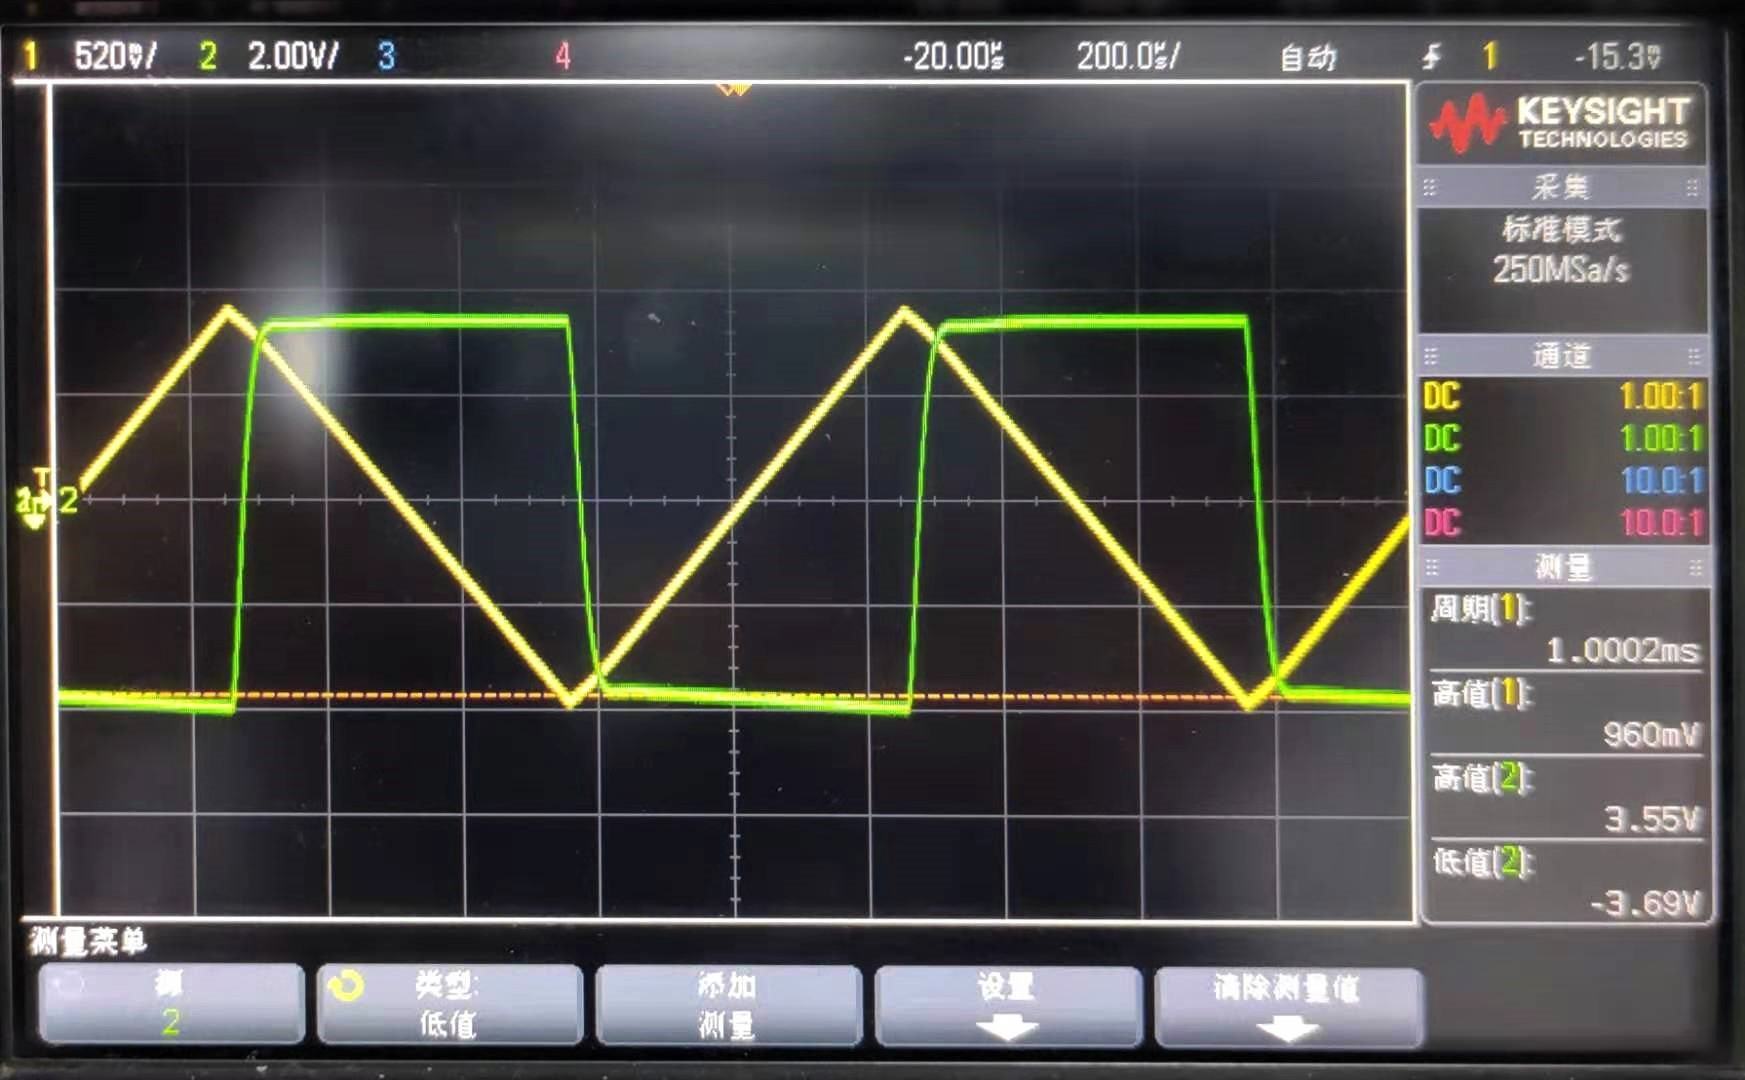
\includegraphics[width=7cm]{Exp06Real}
 \caption{实验六在示波器上的实际输入输出波形}
 \label{fig:Exp06Real}
\end{figure}
\subsubsection{实验分析}
电位器的电阻实际值在 $200\Omega$ 以内,因此相较于 $R_F$ 来说很小。而且考虑到:
\[ v_1=i_1R_1=R_1C\frac{\dd v_c}{\dd t} \]
在 $R_1\sim100\Omega,~C\sim0.1\mr{\upmu F}$量级下非常小,因此可以忽略。
\par 时间常数为:
\[ \tau=R_FC=9.722\mr{k}\Omega\times0.095\mr{\upmu F}=0.924\mr{ms} \]
\par 理论的方波高电平为:
\[ v_o=-R_FC\frac{\dd v_i}{\dd t}=3.644\mr{V} \]
\par 理论的方波低电平为:
\[ v_o=-R_FC\frac{\dd v_i}{\dd t}=-3.644\mr{V} \]
\par 方波高峰值的误差不算太大,大概是 0.04V 左右,这可以用测量误差来解释。但是低峰值达到了 -3.85V ,这显然是不合理的。但是因为某些原因,方波的低处并不水平,有一明显的倾斜。如果改为测量方波低线的中点位置,那么其值大约在 -3.69V 左右,这样绝对误差误差小了许多,还算可以接受。
\par 方波高处低处都不水平,低处倾斜明显一些,而且都是往峰值更大的方向倾斜。考虑到输出电压与电流成正比,这种现象可能是因为:在输入电平不断变化时,非理想的运放总是需要给出电流来跟上这种变化。结果就是,流过 $R_F$ 的电流随着时间得到越来越大的补充(但是补充值相对于原电流值本身还是很小),电压峰值因此微微上涨。
\par 上升沿下降沿不是垂直的,这是因为加入了电阻 $R_1$ 。这使得电容两端电压也需要弛豫一段时间才能达到 $v_i$ 。但是因为 $R_1$ 很小,这个弛豫时间比较短,所以体现出的是一条斜率很大的指数函数曲线,这和示波器上的上升沿下降沿曲线是吻合的。如果 $R_1$ 更大,那么时间常数增大,上升沿下降沿会进一步变差,而且同时方波占空比也下降了,可能使得高处低处难以达到峰值(上升沿还没结束下降沿就开始了);如果 $R_1$ 更小,那么电流变化剧烈,使得 $v_o$ 变化剧烈,会出现振铃现象,在上升沿下降沿之后会有一个振荡指数衰减的图像,这影响了方波的形状,同时可能使得电路在某一瞬间过负载(因为上冲电压大于高峰值)。
\par 所以这个输出图像,是在尽量避免振铃和尽量使上升沿下降沿更好的情况下调整 $R_1$ 得到的。很难得到理想的方波图像。

\section{实验总结}
运算放大器是一种深度反馈有源器件。利用它的虚短和虚断特性,可以构建很多有用的电路,以达到放大、反相、跟随(但提高负载能力)、加法运算、减法运算、积分运算、微分运算等目的。
\par 同时通过本次实验,我们也清楚地认识到,设计出来的电路和实现的电路完全不是一回事。实际运放并没有那么理想,使用的电阻、电容值也未必等于标称值,还有电路中自然存在的电容电感电阻、噪声等,使得电路的性能受到一定影响,甚至影响正常使用。同时我们也找到了一些调整办法来尽量使得电路能够正常工作(比如实验六),并得到了误差范围内正常工作的有效电路。

\section{实验思考题}


\end{document}
